\chapter{Hauptkapitel\#1}

Jedes Kapitel sollte mit einer Kapiteleinleitung beginnen, die als Orientierungshilfe den Inhalt des Kapitels zusammenfasst und wesentliche Punkte hervorhebt.

Entwicklungsorientierte Abschlussarbeiten folgen im Hauptteil der Thesis häufig dem Phasenmodell des Software-Engineerings\footnote{Auch wenn die Arbeit (Erkenntnisse, Entwicklung, Programmierung, \ldots) in anderer
zeitlicher Reihenfolge gewonnen wurden, macht es aus didaktischen Gründen Sinn, dem Phasenmodell zu folgen, da es bekannt und üblich ist und so die Leser:innen die Arbeit leichter verstehen können.}, die jeweils in einem Kapitel ausgeführt werden können:
\begin{itemize}\setlength{\parskip}{1ex}

\item Analyse\\
Die Analyse umfasst zwei wesentliche Fragestellungen: a) die \emph{Ist-Analyse} in der der vorgefundene Zustand dargelegt wird. b) die \emph{Anforderungs-Analyse} die die durch das Projekt umzusetzenden 
funktionalen und nicht-funktionalen Anforderungen erläutert.

\item Design (Entwurf)\\
Der Entwurf stellte die Architektur der Lösung und ihre grundsätzliche, informationstechnische Herangehensweise vor. 
Zentrales Element kann eine graphische Darstellung der beteiligten Komponenten und ihrer Interaktionen sein. Auch können benötigte Algorithmen auf abstrakter Ebene dargestellt werden.

\item Implementierung\\
Die Implementierung führt konkrete Programme oder Konfigurationen vor. Essentieller Programmcode, der die wesentlichen Herausforderungen umsetzte, wird in Auszügen diskutiert.

\item Test (Evaluation, praktischer Einsatz, Messungen)\\
Der Test führt das entstandene System im Einsatz, unter Echtweltbedingungen oder mit Hilfe synthetischer Daten, vor. Hier können ggf.\ auch Screenshots oder relevante Logs diskutiert werden.
\end{itemize}

% Dieses Kapitel konkretisiert die bereits genannten Problematiken, schildert und vergleicht mögliche Umsetzungsvarianten, um diese zu vergleichen und daraus eine Auswahl zu treffen.
Der Hauptteil kann und soll auf die in den Grundlagen vermittelten Begriffe und Sachverhalte zurückgreifen, um das Problem und seine Lösung in angemessener und möglichst verständlicher Weise zu beschreiben.

\section{weitere Layout--Beispiele}

\begin{table}[ht]
\centering
    \begin{tabular}{l r | r}
        \hline\hline
        \thead{Tabelle}
        &
        \thead{\# Einträge}
        &
        \thead{Proz. Anteil der\\ursprünglichen Einträge} \\ [0.5ex] 
        % \thead erlaubt Zeilenumbruch in header
        % [0.5ex] = Abstand zur nächsten Zeile
        \hline
        Face Position Orientation   & $\sim$ 67.847.000 (73.3 \%) &  100.0 \%\\
        Face Demographics           & $\sim$ 24.377.000 (26.3 \%) &   36.0 \%\\
        Image Details               &    $\sim$ 161.000 ( 0.2 \%) &    0.2 \%\\
        Face Details                &    $\sim$ 144.000 ( 0.2 \%) &    0.2 \%\\
        \hline
        \textbf{Gesamt}             &        92.528.750 (100 \%)  &  \\ [1ex]
        \hline\hline
    \end{tabular}
\caption{Verteilung der Einträge auf die gruppierten Tabellen}
\label{tab:verteilung}
\end{table}

\clearpage

\begin{wrapfigure}{l}{0.5\linewidth}
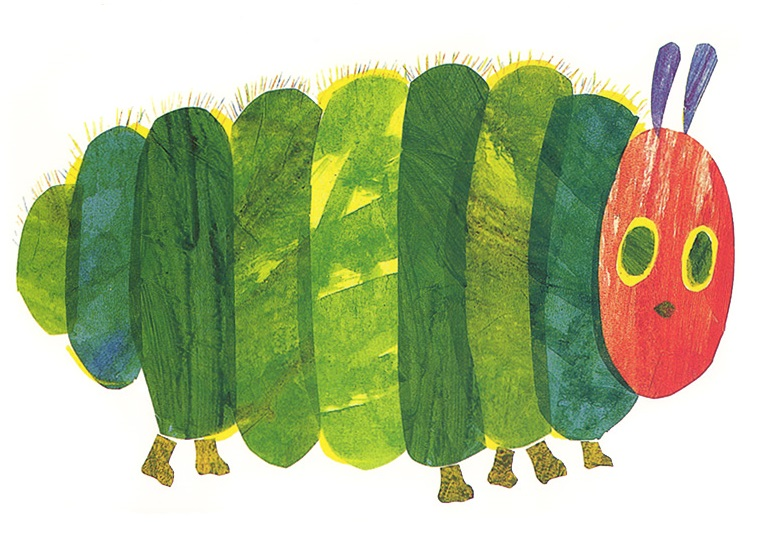
\includegraphics[width=\linewidth]{bilder/caterpillar.jpg}
\caption[Caterpillar]{Caterpillar\cite{caterpillar}}
\label{fig:caterpillar}
\end{wrapfigure}

Lorem ipsum dolor sit amet, consectetur adipiscing elit. Duis blandit, eros vel convallis scelerisque, ante risus hendrerit erat, id luctus urna velit in risus. Nunc nec viverra eros. Duis nisl mi, pharetra non massa ut, scelerisque scelerisque nisi. Donec faucibus nulla id risus condimentum viverra. Aliquam feugiat felis id massa tincidunt, nec malesuada lectus congue. Curabitur sagittis sapien ut augue cursus, eu congue purus sodales. 

Lorem ipsum dolor sit amet, consectetur adipiscing elit. Ut pulvinar viverra mollis. Proin magna justo, congue eget porta ut, maximus vel augue. Donec vehicula leo eu nisi vulputate blandit. Donec ultricies erat in eros suscipit, sit amet mattis elit vulputate. 

\begin{table}[hb]
\scriptsize
\begin{minipage}{0.49\linewidth}
\centering
\begin{tabular}{||c | r | r | r |} 
    \hline
    \textbf{Nr.} & \textbf{\# Ergeb.} & \textbf{PostgreSQL} & \textbf{MongoDB} \\ [0.5ex]
    \hline\hline
    \multirow{3}{*}{1.1} & \multirow{3}{*}{4.678} 
      & 0,9548 s & 0,3056 s \\
    & & 0,8997 s & 0,1290 s \\
    & & 0,9101 s & 0,1213 s \\
    \hline
    \multirow{3}{*}{1.2} & \multirow{3}{*}{4.678} 
      & 1,1088 s & -- \\
    & & 1,2218 s & -- \\
    & & 1,2137 s & -- \\
    \hline
    \multirow{3}{*}{1.3} & \multirow{3}{*}{4.678} 
      & 0,0403 s & -- \\
    & & 0,0412 s & -- \\
    & & 0,0401 s & -- \\
    \hline
    \multirow{3}{*}{2} & \multirow{3}{*}{4.678} 
      & 0,9498 s & 0,1466 s \\
    & & 0,9729 s & 0,1083 s \\
    & & 0,9071 s & 0,1066 s \\
    \hline
    \multirow{3}{*}{3} & \multirow{3}{*}{10.043} 
      & 0,2779 s & 0,3600 s \\
    & & 0,3079 s & 0,2429 s \\
    & & 0,2992 s & 0,2498 s \\
    \hline
    \multirow{3}{*}{4} & \multirow{3}{*}{2} 
      & 0,0018 s & 0,0727 s \\
    & & 0,0009 s & 0,0138 s \\
    & & 0,0009 s & 0,0070 s \\
    \hline
    \multirow{3}{*}{5} & \multirow{3}{*}{253.755}
      & 3,5117 s & 126,0782 s \\
    & & 3,4656 s & 106,1470 s \\
    & & 3,3282 s & 107,9439 s \\
    \hline
\end{tabular}
\end{minipage}
%
\begin{minipage}{0.49\linewidth}
\centering
\begin{tabular}{|c | r | r | r ||} 
    \hline
    \textbf{Nr.} & \textbf{\# Ergeb.} & \textbf{PostgreSQL} & \textbf{MongoDB} \\ [0.5ex] 
    \hline\hline 
    \multirow{3}{*}{6} & \multirow{3}{*}{5.141}
      & 2,1497 s & 12,1915 s \\
    & & 1,8485 s & 11,6134 s \\
    & & 1,7347 s & 11,2647 s \\
    \hline
    \multirow{3}{*}{7} & \multirow{3}{*}{694.907} 
      & 6,3388 s & 23,2439 s \\
    & & 6,6917 s & 22,4676 s \\
    & & 6,6002 s & 22,9043 s \\
    \hline
    \multirow{3}{*}{8} & \multirow{3}{*}{0} 
      & 0,0018 s & 0,0011 s \\
    & & 0,0008 s & 0,0009 s \\
    & & 0,0008 s & 0,0008 s \\
    \hline
    \multirow{3}{*}{9.1} & \multirow{3}{*}{1.635.965} 
      & 27,0328 s & 68,7589 s \\
    & & 28,4229 s & 58,9914 s \\
    & & 27,9176 s & 64,8253 s \\
    \hline
    \multirow{3}{*}{9.2} & \multirow{3}{*}{1.635.965} 
      & 12,2981 s & 73,4722 s \\
    & & 11,5675 s & 63,1674 s \\
    & & 11,4067 s & 68,5112 s \\
    \hline
    \multirow{3}{*}{10.1} & \multirow{3}{*}{14.222.062} 
      & 113,2476 s & 373,5514 s \\
    & & 107,6503 s & 370,8531 s \\
    & & 112,4459 s & 373,4111 s \\
    \hline
    \multirow{3}{*}{10.2} & \multirow{3}{*}{14.222.062} 
      & 143,6760 s & -- \\
    & & 141,0328 s & -- \\
    & & 142,5101 s & -- \\
    \hline
\end{tabular}
\end{minipage}
\caption{Beispieltabelle eines Benchmarks}
\label{tab:benchmark_results}
\end{table}
